% ENSYSTRA (https://ensystra.eu) Report Template
% LaTeX article document class
% customised using 'ensystra-article.sty' by Nithiya Streethran (nmstreethan@gmail.com)
% License: The LaTeX project public license (LPPL), version 1.3c (https://www.latex-project.org/lppl/lppl-1-3c/)
%
% Research and career development plans
% by Nithiya Streethran (nmstreethan@gmail.com)

% DOCUMENT CONFIGURATIONS ---------------------------------------
\documentclass[11pt,twoside]{article}
% define shortcuts to document properties
\def \auth {Nithiya Streethran} % author
\def \doctitle {Documentation} % document title
\def \projtitle {Development of a real-time optimisation solution for dispatchable energy supply units} % project title
\def \uni {University of Stavanger}
\def \keywords {documentation}
\def \dat {\today} % date
\def \email {nmstreethran@gmail.com}
% licenses and copyright notice
\def \licenseurl {https://www.gnu.org/licenses/fdl-1.3} % license URL
\def \copyright {Copyright \textcopyright~\the\year{}~by \auth. Licensed under the GNU Free Documentation License Version 1.3.}

\usepackage{ensystra-article} % custom style with required packages and settings
\addbibresource{References.bib} % bibliography file

%---------------------------------------------------------------
\begin{document}

\maketitle
\tableofcontents
\listoffigures
\listoftables

\section{Preface}
Welcome to the
\href{https://github.com/ENSYSTRA/short-term-forecasting}{short-term-forecasting}
wiki!

Short-term forecasting of electricity generation, demand and prices
using machine learning.

Copyright (C) 2019 Nithiya Streethran.

Permission is granted to copy, distribute and/or modify this document
under the terms of the GNU Free Documentation License, Version 1.3 or
any later version published by the Free Software Foundation; with no
Invariant Sections, no Front-Cover Texts, and no Back-Cover Texts. A
copy of the license is included in the section entitled ``GNU Free
Documentation License''.

Images are licensed under the Creative Commons Attribution-ShareAlike
4.0 International (CC BY-SA 4.0) license, where the image source has not
been specified.

This work is part of Nithiya Streethran's research as Early-Stage
Researcher (ESR) 9 of the \href{https://ensystra.eu/}{ENSYSTRA - ENergy
SYStems in TRAnsition} Innovative Training Network. ENSYSTRA is funded
by the European Union's Horizon 2020 research and innovation programme
under the Marie Skłodowska-Curie grant agreement No: 765515.


\hypertarget{background}{%
\section{Background}\label{background}}

The transition towards a future low-carbon economy is driven globally by
the Paris Agreement {[}Pari15{]}, which recognises the need for
sustainable development worldwide to counter the threats of climate
change. The European Union (EU) is committed to reduce greenhouse gas
(GHG) emissions by 2050 to 80-90 \% below 1990 levels {[}Ener12{]}. As
the energy industry is responsible for the highest share of
anthropogenic GHG emissions, importance is placed on how changes in
energy systems can help achieve these GHG emission reduction targets
{[}Ener12{]}.

A number of opportunities exist for the decarbonisation of the energy
industry. The International Renewable Energy Agency (IRENA), in their
renewable energy roadmap study, has identified renewable energy as
having the highest potential in reducing energy-related carbon dioxide
(CO2) emissions globally, which is closely followed by energy efficiency
and electrification with renewable energy {[}Glob18{]}. In a 2018
political agreement, the EU member states agreed upon a target of at
least 32 \% of the demand being met with renewables by 2030, through
national targets of the individual member states {[}ReneND{]}. The
electricity demand in the transport sector is also expected to increase
due to expected petrol and diesel engine bans and subsequently the
electrification of road transport {[}Worl17{]}.

The energy system is also transitioning towards a decentralised system
with more consumer participation and new forms of flexibilities,
including sector coupling, demand-side management (DSM), energy
conversion and storage, cross-border interconnection and curtailment.
This allows demand patterns to shift to better suit the generation
patterns in systems with high penetration of variable renewable energy
(VRE) resources, such as solar and wind {[}Lund17{]}, {[}Towa18{]}.
However, this requires cooperation involving many actors with various
responsibilities and dependencies that interact within this energy
system, and opens up the opportunity to perform interdisciplinary
research work in the area of energy system analysis.

The ENSYSTRA - ENergy SYStems in TRAnsition Innovative Training Network
has been established to address the challenges of the energy transition
with interdisciplinary collaboration and regional cooperation involving
academia, government and industry {[}AbouND{]}. ENSYSTRA is centred on
the North Sea region and focusses on performing interdisciplinary
modelling work involving technology, economics, social science and
humanities, and combining various modelling approaches in different
levels and resolutions. ENSYSTRA aims to keep an open science approach,
which will allow the resulting models to be subject to full scientific
scrutiny.

Energy systems models, which are tools used to project the future energy
supply of a country or region {[}Herb12{]}, is the centre of ENSYSTRA.
The figure below explains the energy systems modelling process using a
system analysis approach {[}Kroo15{]}. This process starts with creating
a model of the actual energy system by simplifying and conceptualising
the present system. This conceptualised system with all assumptions is
then mathematically solved to produce numerical results. These results
can then be interpreted and conclusions can be drawn regarding the
future energy system. Such conclusions form the evidence-base for
decision makers, resulting in policy implications or operational
strategies that help achieve these climate targets.

\begin{figure}
\centering
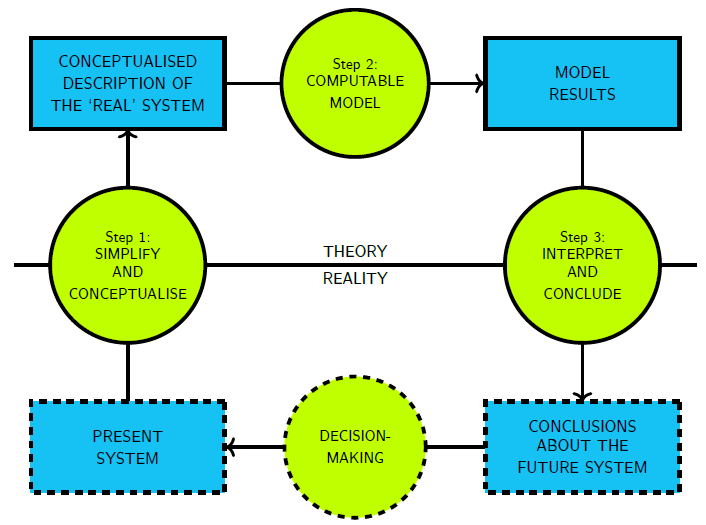
\includegraphics{images/system-analysis.png}
\caption{The system analysis approach applied on the energy system
modelling process, adapted from Krook-Riekkola 2015 {[}Kroo15{]}.}
\end{figure}

There are 15 early-stage researchers (ESRs) across four work packages
(WPs) in ENSYSTRA, as shown in the figure below. The research project
entitled ``Development of a real-time optimisation solution for
dispatchable energy supply units'' is conducted by ESR 9, who is
enrolled as a PhD student at University of Stavanger (UiS) in Norway.
This project is within WP 2 (technology prospects and development
pathways), which focusses on technological options for the energy
transition, mainly in terms of techno-economic performance over time.
For this research project, the technology focus is on the digitalisation
of the electricity sector. As the electricity system transitions into
smart systems, the system will have an increasing amount of sensors and
controllers that continuously record measurements of the system
{[}Lund17{]}. Advancements in these technologies mean that data that is
fast, heterogeneous and high in volume from the electricity system will
be generated. Data with these characteristics must be managed and
analysed effectively to gain insights on the electricity system, which
can then be converted to strategies that optimise the system
{[}Mana12{]}. This project will specifically investigate how artificial
intelligence (AI) can play a role in the transition to a low-carbon
electricity system by utilising high resolution data of the system. The
next section will investigate this, as well as explain what is meant by
``real-time'' and ``dispatchable'' in the context of electricity systems
in this project.

\begin{figure}
\centering
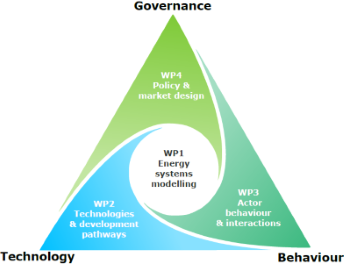
\includegraphics{images/wp.png}
\caption{Interactions between the four WPs of the ENSYSTRA project.
Source: ENSYSTRA {[}AbouND{]}.}
\end{figure}

\hypertarget{problem-definition}{%
\section{Problem definition}\label{problem-definition}}

The table below shows the characteristics of the main energy generation
technologies, including their costs. These generation sources have
different variabilities, fuel types, flexibilities, costs and carbon
emissions. According to the EU reference scenario 2016 {[}EnerND{]},
wind and solar energy resources, which are VRE resources, are expected
to generate a total of 35 \% of EU's electricity by 2050, which is a
significant increase (23 \%) from 2015 levels. Conversely, generation
from nuclear and solids, which are not variable and provide base load
generation, are expected to decrease significantly. Unlike conventional
generators, VRE are intermittent as they are dependent on atmospheric
conditions, such as wind speed and cloud cover, and they vary spatially
(i.e., location-dependent) and temporally {[}Josk11{]}. Therefore, VRE
generation cannot be controlled to meet the demand patterns and needs of
the energy system {[}Josk11{]}, which is a challenge to electricity and
energy system operators in general.

\begin{longtable}[]{@{}llllllll@{}}
\caption{Characteristics of the main energy generation technologies,
adapted from Erbach 2016 {[}Erba16{]} and Tidball, et al.~2010
{[}Tidb10{]}.}\tabularnewline
\toprule
Type\protect\hyperlink{f1}{{[}f1{]}} & Variable & Fuel type &
Flexibility & Low carbon & CAPEX\protect\hyperlink{f2}{{[}f2{]}} &
OPEX\protect\hyperlink{f2}{{[}f2{]}} &
LCOE\protect\hyperlink{f2}{{[}f2{]}}\tabularnewline
\midrule
\endfirsthead
\toprule
Type\protect\hyperlink{f1}{{[}f1{]}} & Variable & Fuel type &
Flexibility & Low carbon & CAPEX\protect\hyperlink{f2}{{[}f2{]}} &
OPEX\protect\hyperlink{f2}{{[}f2{]}} &
LCOE\protect\hyperlink{f2}{{[}f2{]}}\tabularnewline
\midrule
\endhead
Coal & no & fossil & medium & no & low & high & very low\tabularnewline
Natural gas & no & fossil & high & no & very low & very high &
low\tabularnewline
Biomass & no & renewable & medium & yes\protect\hyperlink{f3}{{[}f3{]}}
& low & very high & very high\tabularnewline
Nuclear & no & nuclear & low & zero-emission & medium & medium &
medium\tabularnewline
Hydro & no & renewable & very high & zero-emission & & &\tabularnewline
Solar & yes & renewable & very low & zero-emission & very high & very
low & very high\tabularnewline
Wind & yes & renewable & very low & zero-emission & & &\tabularnewline
\emph{Onshore wind} & & & & & high & very low & very low\tabularnewline
\emph{Offshore wind} & & & & & very high & low & high\tabularnewline
Geothermal & no & renewable & high & zero-emission & high & medium &
high\tabularnewline
\bottomrule
\end{longtable}

{[}f1{]} \emph{Costs for natural gas, biomass, solar and geothermal are
that of advanced combustion turbine, biomass gasification plant,
utility-scale photovoltaic and hydrothermal plant respectively}

{[}f2{]} \emph{CAPEX - capital costs; OPEX - operational expenditure
(includes fuel and fixed O\&M costs); LCOE - levelised cost of
electricity}

{[}f3{]} \emph{regrowth of biomass compensates emissions}

\hypertarget{objectives}{%
\section{Objectives}\label{objectives}}

The main research objective of this project is:

\begin{quote}
\emph{To develop an open-source, machine learning-based electricity
market model for the North Sea region which will help electricity
generators, retailers, large consumers, BRPs and system operators in
short-term electricity markets (i.e., day-ahead and intra-day markets)
to develop operational and bidding strategies that maximise their
profits under uncertainty of VRE generation. The model will consist of a
forecaster based on machine learning, which will use high resolution
time series weather forecasts for the upcoming period, and recent
historical measurements of electricity generation, demand and market
prices, to forecast the latter three quantities for the upcoming period.
These forecasts will serve as inputs to an optimiser, which maximises
social welfare in the electricity market.}
\end{quote}

Based on the main research objective, the following research questions
have been derived:

\begin{itemize}
\tightlist
\item
  What methods and resources are needed to process and store the large
  volume of high resolution data required for this model?
\item
  What type of machine learning algorithms are suited for the time
  series forecasting of electricity prices, demand and generation?
\item
  What optimisation methods are suitable for maximising the social
  welfare problem in the electricity market, and what are the
  constraints to this optimisation problem?
\item
  What methods can be used to analyse the inputs and outputs of the
  model and translate them into operational strategies relevant to the
  market participant?
\item
  How can this model be standardised and published so that it is
  available for use openly by any participant in the electricity market,
  as well as other interested parties, such as policymakers?
\item
  How can this high resolution electricity market operational model be
  integrated with the overall North Sea energy systems model to provide
  insights on long-term planning and investments in the energy sector?
\end{itemize}

\hypertarget{regions}{%
\section{Regions}\label{regions}}

\hypertarget{north-sea-countries}{%
\subsection{North Sea countries}\label{north-sea-countries}}

As per the definition provided by the European MSP Platform {[}NortND{]}
and the CPMR North Sea Commission {[}Memb15{]}, the North Sea region
consists of eight countries: Belgium, Denmark, France, Germany,
Netherlands, Norway, Sweden and United Kingdom.

\hypertarget{nuts-nomenclature-of-territorial-units-for-statistics}{%
\subsubsection{\texorpdfstring{\href{https://ec.europa.eu/eurostat/web/nuts/background}{NUTS
(Nomenclature of territorial units for
statistics)}}{NUTS (Nomenclature of territorial units for statistics)}}\label{nuts-nomenclature-of-territorial-units-for-statistics}}

\href{https://github.com/ENSYSTRA/short-term-forecasting/tree/master/jupyter-notebooks/NUTS.ipynb}{See
the Jupyter notebook}.

\hypertarget{bidding-zones}{%
\subsection{Bidding zones}\label{bidding-zones}}

\hypertarget{definition}{%
\subsubsection{Definition}\label{definition}}

According to {[}Bidd14{]}:

\begin{itemize}
\tightlist
\item
  The largest geographical area within which market participants are
  able to exchange energy without capacity allocation.
\item
  The majority of bidding zones in Europe are defined by national
  borders (e.g., France or the Netherlands).
\item
  Some are larger than national borders (e.g., Austria, Germany and
  Luxembourg or the Single Electricity Market for the island of Ireland)
\item
  Some are smaller zones within individual countries (e.g., Italy,
  Norway or Sweden).
\end{itemize}

\hypertarget{bidding-zones-in-the-north-sea-region}{%
\subsubsection{Bidding zones in the North Sea
region}\label{bidding-zones-in-the-north-sea-region}}

The bidding zones in the European electricity market are illustrated in
the map below {[}Tren17{]}.

\begin{figure}
\centering
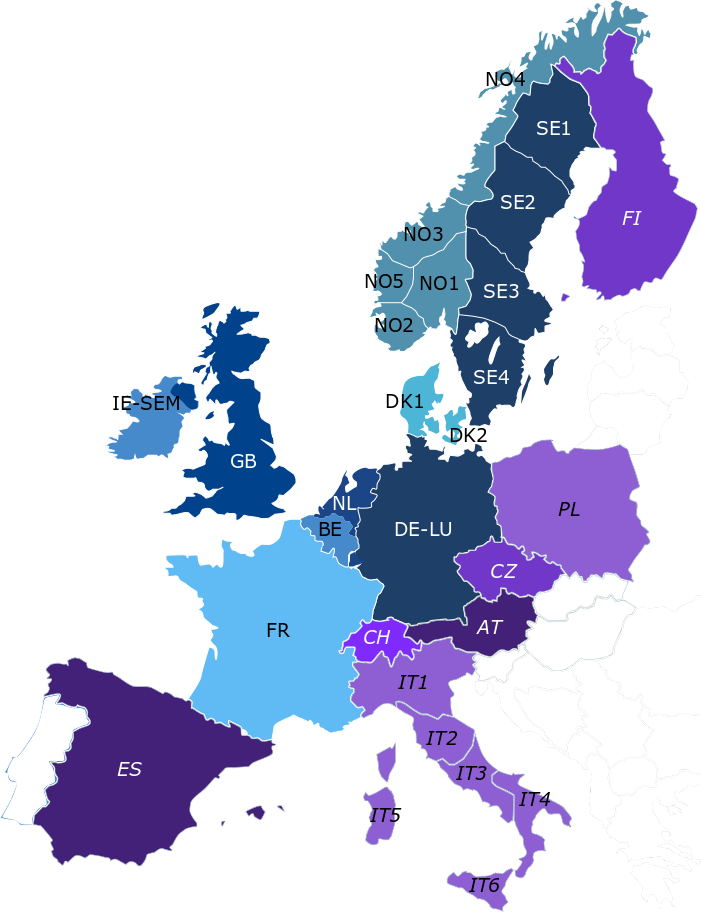
\includegraphics{images/market-map.png}
\caption{Bidding zones in the European electricity market. Source:
\href{http://raport.pse.pl/en/trends-and-market-context}{Polskie Sieci
Elektroenergetyczne} {[}Tren17{]}.}
\end{figure}

\begin{longtable}[]{@{}lll@{}}
\caption{Bidding zones in the North Sea region.}\tabularnewline
\toprule
\textbf{Country} & \textbf{Market(s)} & \textbf{Zone(s)}\tabularnewline
\midrule
\endfirsthead
\toprule
\textbf{Country} & \textbf{Market(s)} & \textbf{Zone(s)}\tabularnewline
\midrule
\endhead
Belgium (BE) & EPEX SPOT & BE\tabularnewline
Germany (DE / GE) & EPEX SPOT &
DE-AT-LU\protect\hyperlink{f4}{{[}f4{]}}\tabularnewline
Denmark (DK) & Nord Pool & DK1, DK2\tabularnewline
France (FR) & EPEX SPOT & FR\tabularnewline
Netherlands (NL) & EPEX SPOT & NL\tabularnewline
Norway (NO) & Nord Pool & NO1, NO2, NO3, NO4, NO5\tabularnewline
Sweden (SE / SW) & Nord Pool & SE1, SE2, SE3, SE4\tabularnewline
United Kingdom (UK) & EPEX SPOT, Nord Pool & GB,
I-SEM\protect\hyperlink{f4}{{[}f4{]}}\tabularnewline
\bottomrule
\end{longtable}

{[}f4{]} \emph{Austria (AT / AU); Luxembourg (LU); Great Britain (GB);
Irish single electricity market (I-SEM), which includes Republic of
Ireland (IE) and UK's Northern Ireland (NI).}

\hypertarget{transmission-system-operators-and-interconnections}{%
\subsubsection{Transmission system operators and
interconnections}\label{transmission-system-operators-and-interconnections}}

The power exchanges that operate in the North Sea region are EPEX SPOT
(Belgium, France, Germany, Netherlands, United Kingdom) and Nord Pool
(Denmark, Norway, Sweden, United Kingdom) {[}Over16{]}, {[}See ND{]},
{[}EPEXND{]}. The day-ahead market takes place generally as an hourly
auction 24 hours prior to dispatch {[}Over16{]}. The intra-day market
has continuous trading and will operate until two hours and up to five
minutes before dispatch {[}Over16{]}. The North Sea region consists of
multiple TSOs, cross-border interconnections and bidding zones, as
listed in the table below.

\begin{longtable}[]{@{}llll@{}}
\caption{TSOs and cross-border interconnections in the North Sea region.
Data: European Network of Transmission System Operators for Electricity
{[}ENTSND{]}, {[}RegiND{]}.}\tabularnewline
\toprule
\begin{minipage}[b]{0.07\columnwidth}\raggedright
Ctry.\protect\hyperlink{f5}{{[}f5{]}}\strut
\end{minipage} & \begin{minipage}[b]{0.37\columnwidth}\raggedright
TSOs\strut
\end{minipage} & \begin{minipage}[b]{0.22\columnwidth}\raggedright
Cross-border
interconnection\protect\hyperlink{f5}{{[}f5{]}},\protect\hyperlink{f6}{{[}f6{]}}\strut
\end{minipage} & \begin{minipage}[b]{0.22\columnwidth}\raggedright
Bidding
zones\protect\hyperlink{f5}{{[}f5{]}},\protect\hyperlink{f6}{{[}f6{]}}\strut
\end{minipage}\tabularnewline
\midrule
\endfirsthead
\toprule
\begin{minipage}[b]{0.07\columnwidth}\raggedright
Ctry.\protect\hyperlink{f5}{{[}f5{]}}\strut
\end{minipage} & \begin{minipage}[b]{0.37\columnwidth}\raggedright
TSOs\strut
\end{minipage} & \begin{minipage}[b]{0.22\columnwidth}\raggedright
Cross-border
interconnection\protect\hyperlink{f5}{{[}f5{]}},\protect\hyperlink{f6}{{[}f6{]}}\strut
\end{minipage} & \begin{minipage}[b]{0.22\columnwidth}\raggedright
Bidding
zones\protect\hyperlink{f5}{{[}f5{]}},\protect\hyperlink{f6}{{[}f6{]}}\strut
\end{minipage}\tabularnewline
\midrule
\endhead
\begin{minipage}[t]{0.07\columnwidth}\raggedright
BE\strut
\end{minipage} & \begin{minipage}[t]{0.37\columnwidth}\raggedright
Elia System Operator\strut
\end{minipage} & \begin{minipage}[t]{0.22\columnwidth}\raggedright
FR, LU, NL, UK\strut
\end{minipage} & \begin{minipage}[t]{0.22\columnwidth}\raggedright
BE\strut
\end{minipage}\tabularnewline
\begin{minipage}[t]{0.07\columnwidth}\raggedright
DK\strut
\end{minipage} & \begin{minipage}[t]{0.37\columnwidth}\raggedright
Energinet\strut
\end{minipage} & \begin{minipage}[t]{0.22\columnwidth}\raggedright
DE, NO, SE\strut
\end{minipage} & \begin{minipage}[t]{0.22\columnwidth}\raggedright
DK1, DK2\strut
\end{minipage}\tabularnewline
\begin{minipage}[t]{0.07\columnwidth}\raggedright
DE\strut
\end{minipage} & \begin{minipage}[t]{0.37\columnwidth}\raggedright
TransnetBW, TenneT TSO, Amprion, 50Hertz Transmission\strut
\end{minipage} & \begin{minipage}[t]{0.22\columnwidth}\raggedright
AT, CH, CZ, DK, FR, LU, NL, PL, SE\strut
\end{minipage} & \begin{minipage}[t]{0.22\columnwidth}\raggedright
CZ+DE+SK, DE-AT-LU, DE-LU\strut
\end{minipage}\tabularnewline
\begin{minipage}[t]{0.07\columnwidth}\raggedright
FR\strut
\end{minipage} & \begin{minipage}[t]{0.37\columnwidth}\raggedright
Réseau de Transport d'Electricité\strut
\end{minipage} & \begin{minipage}[t]{0.22\columnwidth}\raggedright
BE, CH, DE, ES, IT, UK\strut
\end{minipage} & \begin{minipage}[t]{0.22\columnwidth}\raggedright
FR\strut
\end{minipage}\tabularnewline
\begin{minipage}[t]{0.07\columnwidth}\raggedright
NL\strut
\end{minipage} & \begin{minipage}[t]{0.37\columnwidth}\raggedright
TenneT TSO\strut
\end{minipage} & \begin{minipage}[t]{0.22\columnwidth}\raggedright
BE, DE, NO, UK\strut
\end{minipage} & \begin{minipage}[t]{0.22\columnwidth}\raggedright
NL\strut
\end{minipage}\tabularnewline
\begin{minipage}[t]{0.07\columnwidth}\raggedright
NO\strut
\end{minipage} & \begin{minipage}[t]{0.37\columnwidth}\raggedright
Statnett\strut
\end{minipage} & \begin{minipage}[t]{0.22\columnwidth}\raggedright
DK, FI, NL, SE\strut
\end{minipage} & \begin{minipage}[t]{0.22\columnwidth}\raggedright
NO1, NO2, NO3, NO4, NO5\strut
\end{minipage}\tabularnewline
\begin{minipage}[t]{0.07\columnwidth}\raggedright
SE\strut
\end{minipage} & \begin{minipage}[t]{0.37\columnwidth}\raggedright
Svenska Kraftnät\strut
\end{minipage} & \begin{minipage}[t]{0.22\columnwidth}\raggedright
DK, FI, DE, LT, NO, PL\strut
\end{minipage} & \begin{minipage}[t]{0.22\columnwidth}\raggedright
SE1, SE2, SE3, SE4\strut
\end{minipage}\tabularnewline
\begin{minipage}[t]{0.07\columnwidth}\raggedright
UK\strut
\end{minipage} & \begin{minipage}[t]{0.37\columnwidth}\raggedright
National Grid Electricity Transmission, System Operator for Northern
Ireland, Scottish Hydro Electric Transmission, ScottishPower
Transmission\strut
\end{minipage} & \begin{minipage}[t]{0.22\columnwidth}\raggedright
BE, FR, IE, NL\strut
\end{minipage} & \begin{minipage}[t]{0.22\columnwidth}\raggedright
GB, IE (SEM)\strut
\end{minipage}\tabularnewline
\bottomrule
\end{longtable}

{[}f5{]} \emph{Ctry. - Country; AT - Austria; BE - Belgium; CH -
Switzerland; CZ - Czech Republic; DE - Germany; DK - Denmark; ES -
Spain; FI - Finland; FR - France; GB - Great Britain; IE - Ireland; IT -
Italy; LT - Lithuania; LU - Luxembourg; NL - Netherlands; NO - Norway;
PL - Poland; SE - Sweden; SK - Slovakia; UK - United Kingdom; SEM -
Single electricity market.}

{[}f6{]} \emph{These countries are not part of the North Sea region: AT,
CH, CZ, ES, FI, IE, IT, LT, LU, PL.}

\hypertarget{data}{%
\section{Data}\label{data}}

\hypertarget{data-folder-navigation}{%
\subsection{\texorpdfstring{\href{https://drive.google.com/drive/folders/1_3Y30j_c-4iai0WuhcrysXHYdZ4F2AKB}{Data
folder}
navigation}{Data folder navigation}}\label{data-folder-navigation}}

\begin{itemize}
\tightlist
\item
  ENTSO-E

  \begin{itemize}
  \tightlist
  \item
    generation and load data for each bidding zone in the North Sea
    region, grouped by country
  \end{itemize}
\item
  Meteo - meteorological data, grouped by country
\item
  Market - market data for the North Sea region
\item
  NUTS - territorial units
\item
  output - output or modified data from this project
\end{itemize}

\hypertarget{met-data}{%
\subsection{Met data}\label{met-data}}

\hypertarget{deutscher-wetterdienst}{%
\paragraph{\texorpdfstring{\href{https://www.dwd.de/EN/climate_environment/cdc/cdc_node.html}{Deutscher
Wetterdienst}}{Deutscher Wetterdienst}}\label{deutscher-wetterdienst}}

\begin{itemize}
\tightlist
\item
  \href{https://cdc.dwd.de/portal/}{CDC (Climate Data Center) portal}
\item
  \href{https://opendata.dwd.de/climate_environment/CDC/}{CDC OpenData}
\item
  \href{https://opendata.dwd.de/climate_environment/CDC/Terms_of_use.pdf}{Terms
  of use for data on the CDC ftp server}
\item
  Data set descriptions

  \begin{itemize}
  \tightlist
  \item
    \href{https://cdc.dwd.de/sdi/pid/TT_TU_MN009/DESCRIPTION_TT_TU_MN009_en.pdf}{Hourly
    station observations of air temperature at 2 m above ground in °C
    for Germany}
  \item
    \href{https://cdc.dwd.de/sdi/pid/RF_TU_MN009/DESCRIPTION_RF_TU_MN009_en.pdf}{Hourly
    station observations of relative humidity in \% for Germany}
  \item
    \href{https://cdc.dwd.de/sdi/pid/R1_MN008/DESCRIPTION_R1_MN008_en.pdf}{Hourly
    station observations of precipitation amount in mm for Germany}
  \item
    \href{https://cdc.dwd.de/sdi/pid/WRTR_MN008/DESCRIPTION_WRTR_MN008_en.pdf}{Hourly
    station observations of form of precipitation (WR code) for Germany}
  \item
    \href{https://cdc.dwd.de/sdi/pid/RS_IND_MN008/DESCRIPTION_RS_IND_MN008_en.pdf}{Hourly
    station observations of index whether precipitation has fallen for
    Germany}
  \item
    \href{https://cdc.dwd.de/sdi/pid/F_MN003/DESCRIPTION_F_MN003_en.pdf}{Hourly
    mean of station observations of wind speed ca. 10 m above ground in
    m/s for Germany}
  \item
    \href{https://cdc.dwd.de/sdi/pid/D_MN003/DESCRIPTION_D_MN003_en.pdf}{Hourly
    mean of station observations of wind direction at ca. 10 m above
    ground in degree for Germany}
  \item
    \href{https://cdc.dwd.de/sdi/pid/P0_MN008/DESCRIPTION_P0_MN008_en.pdf}{Hourly
    station observations of air pressure at station level in hpa for
    Germany}
  \item
    \href{https://cdc.dwd.de/sdi/pid/P_MN008/DESCRIPTION_P_MN008_en.pdf}{Hourly
    station observations of air pressure at mean sea level in hpa for
    Germany}
  \item
    \href{https://cdc.dwd.de/sdi/pid/N_MN008/DESCRIPTION_N_MN008_en.pdf}{Hourly
    station observations of cloud coverage in eighths for Germany}
  \end{itemize}
\item
  \href{https://opendata.dwd.de/climate_environment/CDC/observations_germany/climate/hourly/wind/}{Hourly
  wind data}
\end{itemize}

\hypertarget{royal-netherlands-meteorological-institute}{%
\paragraph{\texorpdfstring{\href{https://data.knmi.nl/datasets}{Royal
Netherlands Meteorological
Institute}}{Royal Netherlands Meteorological Institute}}\label{royal-netherlands-meteorological-institute}}

\hypertarget{met-office}{%
\paragraph{\texorpdfstring{\href{https://www.metoffice.gov.uk/datapoint}{Met
Office}}{Met Office}}\label{met-office}}

\hypertarget{norwegian-meteorological-institute}{%
\paragraph{\texorpdfstring{\href{https://www.met.no/en/free-meteorological-data}{Norwegian
Meteorological
Institute}}{Norwegian Meteorological Institute}}\label{norwegian-meteorological-institute}}

\hypertarget{swedish-meteorological-and-hydrological-institute}{%
\paragraph{\texorpdfstring{\href{https://www.smhi.se/en/services/professional-services/data-and-statistics}{Swedish
Meteorological and Hydrological
Institute}}{Swedish Meteorological and Hydrological Institute}}\label{swedish-meteorological-and-hydrological-institute}}

\hypertarget{danish-meteorological-institute}{%
\paragraph{\texorpdfstring{\href{http://research.dmi.dk/data/}{Danish
Meteorological
Institute}}{Danish Meteorological Institute}}\label{danish-meteorological-institute}}

\hypertarget{muxe9tuxe9o-france}{%
\paragraph{\texorpdfstring{\href{https://donneespubliques.meteofrance.fr/}{Météo-France}}{Météo-France}}\label{muxe9tuxe9o-france}}

\hypertarget{the-royal-meteorological-institute-of-belgium}{%
\paragraph{\texorpdfstring{\href{https://opendata.meteo.be/}{The Royal
Meteorological Institute of
Belgium}}{The Royal Meteorological Institute of Belgium}}\label{the-royal-meteorological-institute-of-belgium}}

\hypertarget{generation-and-demand-data}{%
\subsection{Generation and demand
data}\label{generation-and-demand-data}}

\hypertarget{entso-e-transparency-platform}{%
\paragraph{\texorpdfstring{\href{https://transparency.entsoe.eu/}{ENTSO-E
Transparency
Platform}}{ENTSO-E Transparency Platform}}\label{entso-e-transparency-platform}}

\begin{itemize}
\tightlist
\item
  \href{https://docstore.entsoe.eu/Documents/MC\%20documents/Transparency\%20Platform/ENTSOE_Transparency_Terms_Conditions.pdf}{GENERAL
  TERMS AND CONDITIONS FOR THE USE OF THE ENTSO-E TRANSPARENCY PLATFORM}
\item
  \href{https://docstore.entsoe.eu/Documents/MC\%20documents/Transparency\%20Platform/List_of_Data_available_for_reuse.pdf}{LIST
  OF DATA AVAILABLE FOR FREE RE-USE}
\item
  Downloaded data:

  \begin{itemize}
  \tightlist
  \item
    \href{https://transparency.entsoe.eu/generation/r2/actualGenerationPerProductionType/show}{Actual
    Generation per Production Type}
  \item
    \href{https://transparency.entsoe.eu/load-domain/r2/totalLoadR2/show}{Total
    Load - Day Ahead / Actual}
  \end{itemize}
\end{itemize}

\hypertarget{market-data}{%
\subsection{Market data}\label{market-data}}

\hypertarget{nord-pool}{%
\paragraph{\texorpdfstring{\href{https://www.nordpoolgroup.com/historical-market-data/}{Nord
Pool}}{Nord Pool}}\label{nord-pool}}

\begin{itemize}
\tightlist
\item
  \href{https://www.nordpoolgroup.com/trading/join-our-markets/membership/}{Membership
  list - Nord Pool}
\item
  \href{https://www.nordpoolgroup.com/About-us/Terms-and-conditions-for-use/}{Terms
  and conditions for use}
\end{itemize}

\hypertarget{epex-spot}{%
\paragraph{\texorpdfstring{\href{https://www.epexspot.com/en/extras/download-center/market_data}{EPEX
Spot}}{EPEX Spot}}\label{epex-spot}}

\begin{itemize}
\tightlist
\item
  \href{https://www.epexspot.com/en/membership/list_of_members}{EPEX
  SPOT Exchange Members}
\end{itemize}

\hypertarget{other-data}{%
\subsection{Other data}\label{other-data}}

\hypertarget{nuts-nomenclature-of-territorial-units-for-statistics}{%
\paragraph{\texorpdfstring{\href{https://ec.europa.eu/eurostat/web/gisco/geodata/reference-data/administrative-units-statistical-units/nuts}{NUTS
(Nomenclature of territorial units for
statistics)}}{NUTS (Nomenclature of territorial units for statistics)}}\label{nuts-nomenclature-of-territorial-units-for-statistics}}

\hypertarget{methodology}{%
\section{Methodology}\label{methodology}}

\hypertarget{modelling-framework}{%
\subsection{Modelling framework}\label{modelling-framework}}

\begin{figure}
\centering
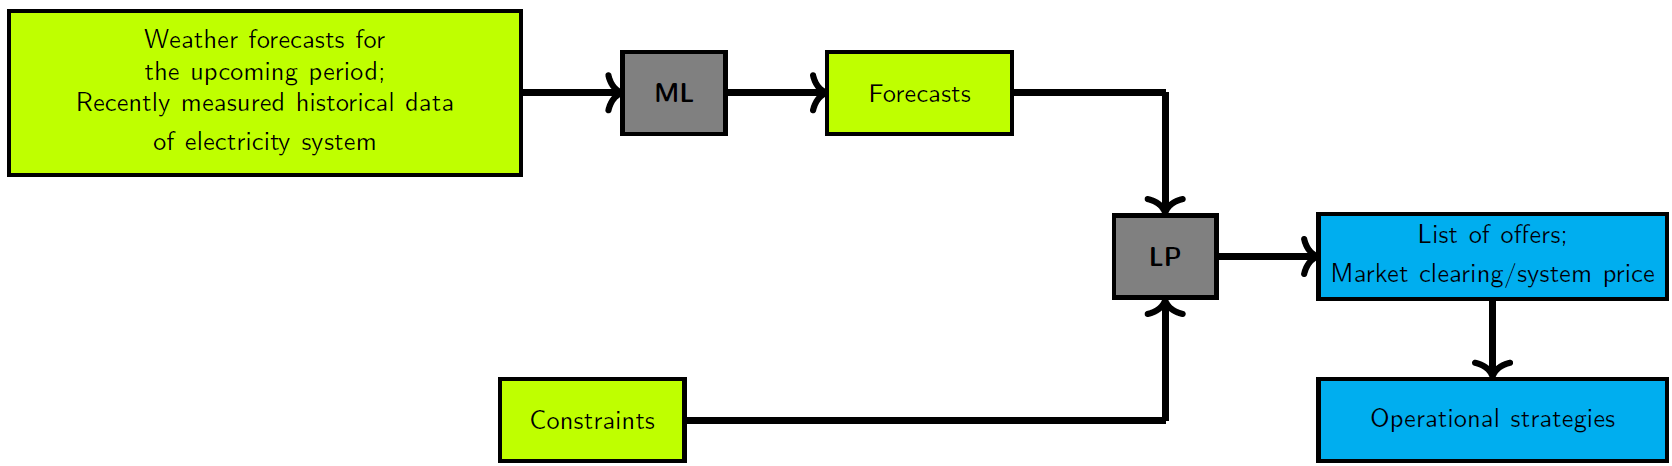
\includegraphics{images/model_framework.png}
\caption{Modelling framework. License: CC BY-SA 4.0.}
\end{figure}


\nocite{*}
\section{References}
\printbibliography[heading=none]

\hypertarget{license}{%
\section{License}\label{license}}

\hypertarget{gnu-free-documentation-license}{%
\subsection{GNU Free Documentation
License}\label{gnu-free-documentation-license}}

Version 1.3, 3 November 2008

Copyright (C) 2000, 2001, 2002, 2007, 2008 Free Software Foundation,
Inc. \url{https://fsf.org/}

Everyone is permitted to copy and distribute verbatim copies of this
license document, but changing it is not allowed.

\hypertarget{preamble}{%
\paragraph{0. PREAMBLE}\label{preamble}}

The purpose of this License is to make a manual, textbook, or other
functional and useful document ``free'' in the sense of freedom: to
assure everyone the effective freedom to copy and redistribute it, with
or without modifying it, either commercially or noncommercially.
Secondarily, this License preserves for the author and publisher a way
to get credit for their work, while not being considered responsible for
modifications made by others.

This License is a kind of ``copyleft'', which means that derivative
works of the document must themselves be free in the same sense. It
complements the GNU General Public License, which is a copyleft license
designed for free software.

We have designed this License in order to use it for manuals for free
software, because free software needs free documentation: a free program
should come with manuals providing the same freedoms that the software
does. But this License is not limited to software manuals; it can be
used for any textual work, regardless of subject matter or whether it is
published as a printed book. We recommend this License principally for
works whose purpose is instruction or reference.

\hypertarget{applicability-and-definitions}{%
\paragraph{1. APPLICABILITY AND
DEFINITIONS}\label{applicability-and-definitions}}

This License applies to any manual or other work, in any medium, that
contains a notice placed by the copyright holder saying it can be
distributed under the terms of this License. Such a notice grants a
world-wide, royalty-free license, unlimited in duration, to use that
work under the conditions stated herein. The ``Document'', below, refers
to any such manual or work. Any member of the public is a licensee, and
is addressed as ``you''. You accept the license if you copy, modify or
distribute the work in a way requiring permission under copyright law.

A ``Modified Version'' of the Document means any work containing the
Document or a portion of it, either copied verbatim, or with
modifications and/or translated into another language.

A ``Secondary Section'' is a named appendix or a front-matter section of
the Document that deals exclusively with the relationship of the
publishers or authors of the Document to the Document's overall subject
(or to related matters) and contains nothing that could fall directly
within that overall subject. (Thus, if the Document is in part a
textbook of mathematics, a Secondary Section may not explain any
mathematics.) The relationship could be a matter of historical
connection with the subject or with related matters, or of legal,
commercial, philosophical, ethical or political position regarding them.

The ``Invariant Sections'' are certain Secondary Sections whose titles
are designated, as being those of Invariant Sections, in the notice that
says that the Document is released under this License. If a section does
not fit the above definition of Secondary then it is not allowed to be
designated as Invariant. The Document may contain zero Invariant
Sections. If the Document does not identify any Invariant Sections then
there are none.

The ``Cover Texts'' are certain short passages of text that are listed,
as Front-Cover Texts or Back-Cover Texts, in the notice that says that
the Document is released under this License. A Front-Cover Text may be
at most 5 words, and a Back-Cover Text may be at most 25 words.

A ``Transparent'' copy of the Document means a machine-readable copy,
represented in a format whose specification is available to the general
public, that is suitable for revising the document straightforwardly
with generic text editors or (for images composed of pixels) generic
paint programs or (for drawings) some widely available drawing editor,
and that is suitable for input to text formatters or for automatic
translation to a variety of formats suitable for input to text
formatters. A copy made in an otherwise Transparent file format whose
markup, or absence of markup, has been arranged to thwart or discourage
subsequent modification by readers is not Transparent. An image format
is not Transparent if used for any substantial amount of text. A copy
that is not ``Transparent'' is called ``Opaque''.

Examples of suitable formats for Transparent copies include plain ASCII
without markup, Texinfo input format, LaTeX input format, SGML or XML
using a publicly available DTD, and standard-conforming simple HTML,
PostScript or PDF designed for human modification. Examples of
transparent image formats include PNG, XCF and JPG. Opaque formats
include proprietary formats that can be read and edited only by
proprietary word processors, SGML or XML for which the DTD and/or
processing tools are not generally available, and the machine-generated
HTML, PostScript or PDF produced by some word processors for output
purposes only.

The ``Title Page'' means, for a printed book, the title page itself,
plus such following pages as are needed to hold, legibly, the material
this License requires to appear in the title page. For works in formats
which do not have any title page as such, ``Title Page'' means the text
near the most prominent appearance of the work's title, preceding the
beginning of the body of the text.

The ``publisher'' means any person or entity that distributes copies of
the Document to the public.

A section ``Entitled XYZ'' means a named subunit of the Document whose
title either is precisely XYZ or contains XYZ in parentheses following
text that translates XYZ in another language. (Here XYZ stands for a
specific section name mentioned below, such as ``Acknowledgements'',
``Dedications'', ``Endorsements'', or ``History''.) To ``Preserve the
Title'' of such a section when you modify the Document means that it
remains a section ``Entitled XYZ'' according to this definition.

The Document may include Warranty Disclaimers next to the notice which
states that this License applies to the Document. These Warranty
Disclaimers are considered to be included by reference in this License,
but only as regards disclaiming warranties: any other implication that
these Warranty Disclaimers may have is void and has no effect on the
meaning of this License.

\hypertarget{verbatim-copying}{%
\paragraph{2. VERBATIM COPYING}\label{verbatim-copying}}

You may copy and distribute the Document in any medium, either
commercially or noncommercially, provided that this License, the
copyright notices, and the license notice saying this License applies to
the Document are reproduced in all copies, and that you add no other
conditions whatsoever to those of this License. You may not use
technical measures to obstruct or control the reading or further copying
of the copies you make or distribute. However, you may accept
compensation in exchange for copies. If you distribute a large enough
number of copies you must also follow the conditions in section 3.

You may also lend copies, under the same conditions stated above, and
you may publicly display copies.

\hypertarget{copying-in-quantity}{%
\paragraph{3. COPYING IN QUANTITY}\label{copying-in-quantity}}

If you publish printed copies (or copies in media that commonly have
printed covers) of the Document, numbering more than 100, and the
Document's license notice requires Cover Texts, you must enclose the
copies in covers that carry, clearly and legibly, all these Cover Texts:
Front-Cover Texts on the front cover, and Back-Cover Texts on the back
cover. Both covers must also clearly and legibly identify you as the
publisher of these copies. The front cover must present the full title
with all words of the title equally prominent and visible. You may add
other material on the covers in addition. Copying with changes limited
to the covers, as long as they preserve the title of the Document and
satisfy these conditions, can be treated as verbatim copying in other
respects.

If the required texts for either cover are too voluminous to fit
legibly, you should put the first ones listed (as many as fit
reasonably) on the actual cover, and continue the rest onto adjacent
pages.

If you publish or distribute Opaque copies of the Document numbering
more than 100, you must either include a machine-readable Transparent
copy along with each Opaque copy, or state in or with each Opaque copy a
computer-network location from which the general network-using public
has access to download using public-standard network protocols a
complete Transparent copy of the Document, free of added material. If
you use the latter option, you must take reasonably prudent steps, when
you begin distribution of Opaque copies in quantity, to ensure that this
Transparent copy will remain thus accessible at the stated location
until at least one year after the last time you distribute an Opaque
copy (directly or through your agents or retailers) of that edition to
the public.

It is requested, but not required, that you contact the authors of the
Document well before redistributing any large number of copies, to give
them a chance to provide you with an updated version of the Document.

\hypertarget{modifications}{%
\paragraph{4. MODIFICATIONS}\label{modifications}}

You may copy and distribute a Modified Version of the Document under the
conditions of sections 2 and 3 above, provided that you release the
Modified Version under precisely this License, with the Modified Version
filling the role of the Document, thus licensing distribution and
modification of the Modified Version to whoever possesses a copy of it.
In addition, you must do these things in the Modified Version:

\begin{itemize}
\tightlist
\item
  A. Use in the Title Page (and on the covers, if any) a title distinct
  from that of the Document, and from those of previous versions (which
  should, if there were any, be listed in the History section of the
  Document). You may use the same title as a previous version if the
  original publisher of that version gives permission.
\item
  B. List on the Title Page, as authors, one or more persons or entities
  responsible for authorship of the modifications in the Modified
  Version, together with at least five of the principal authors of the
  Document (all of its principal authors, if it has fewer than five),
  unless they release you from this requirement.
\item
  C. State on the Title page the name of the publisher of the Modified
  Version, as the publisher.
\item
  D. Preserve all the copyright notices of the Document.
\item
  E. Add an appropriate copyright notice for your modifications adjacent
  to the other copyright notices.
\item
  F. Include, immediately after the copyright notices, a license notice
  giving the public permission to use the Modified Version under the
  terms of this License, in the form shown in the Addendum below.
\item
  G. Preserve in that license notice the full lists of Invariant
  Sections and required Cover Texts given in the Document's license
  notice.
\item
  H. Include an unaltered copy of this License.
\item
  I. Preserve the section Entitled ``History'', Preserve its Title, and
  add to it an item stating at least the title, year, new authors, and
  publisher of the Modified Version as given on the Title Page. If there
  is no section Entitled ``History'' in the Document, create one stating
  the title, year, authors, and publisher of the Document as given on
  its Title Page, then add an item describing the Modified Version as
  stated in the previous sentence.
\item
  J. Preserve the network location, if any, given in the Document for
  public access to a Transparent copy of the Document, and likewise the
  network locations given in the Document for previous versions it was
  based on. These may be placed in the ``History'' section. You may omit
  a network location for a work that was published at least four years
  before the Document itself, or if the original publisher of the
  version it refers to gives permission.
\item
  K. For any section Entitled ``Acknowledgements'' or ``Dedications'',
  Preserve the Title of the section, and preserve in the section all the
  substance and tone of each of the contributor acknowledgements and/or
  dedications given therein.
\item
  L. Preserve all the Invariant Sections of the Document, unaltered in
  their text and in their titles. Section numbers or the equivalent are
  not considered part of the section titles.
\item
  M. Delete any section Entitled ``Endorsements''. Such a section may
  not be included in the Modified Version.
\item
  N. Do not retitle any existing section to be Entitled ``Endorsements''
  or to conflict in title with any Invariant Section.
\item
  O. Preserve any Warranty Disclaimers.
\end{itemize}

If the Modified Version includes new front-matter sections or appendices
that qualify as Secondary Sections and contain no material copied from
the Document, you may at your option designate some or all of these
sections as invariant. To do this, add their titles to the list of
Invariant Sections in the Modified Version's license notice. These
titles must be distinct from any other section titles.

You may add a section Entitled ``Endorsements'', provided it contains
nothing but endorsements of your Modified Version by various
partiesâ€''for example, statements of peer review or that the text has
been approved by an organization as the authoritative definition of a
standard.

You may add a passage of up to five words as a Front-Cover Text, and a
passage of up to 25 words as a Back-Cover Text, to the end of the list
of Cover Texts in the Modified Version. Only one passage of Front-Cover
Text and one of Back-Cover Text may be added by (or through arrangements
made by) any one entity. If the Document already includes a cover text
for the same cover, previously added by you or by arrangement made by
the same entity you are acting on behalf of, you may not add another;
but you may replace the old one, on explicit permission from the
previous publisher that added the old one.

The author(s) and publisher(s) of the Document do not by this License
give permission to use their names for publicity for or to assert or
imply endorsement of any Modified Version.

\hypertarget{combining-documents}{%
\paragraph{5. COMBINING DOCUMENTS}\label{combining-documents}}

You may combine the Document with other documents released under this
License, under the terms defined in section 4 above for modified
versions, provided that you include in the combination all of the
Invariant Sections of all of the original documents, unmodified, and
list them all as Invariant Sections of your combined work in its license
notice, and that you preserve all their Warranty Disclaimers.

The combined work need only contain one copy of this License, and
multiple identical Invariant Sections may be replaced with a single
copy. If there are multiple Invariant Sections with the same name but
different contents, make the title of each such section unique by adding
at the end of it, in parentheses, the name of the original author or
publisher of that section if known, or else a unique number. Make the
same adjustment to the section titles in the list of Invariant Sections
in the license notice of the combined work.

In the combination, you must combine any sections Entitled ``History''
in the various original documents, forming one section Entitled
``History''; likewise combine any sections Entitled
``Acknowledgements'', and any sections Entitled ``Dedications''. You
must delete all sections Entitled ``Endorsements''.

\hypertarget{collections-of-documents}{%
\paragraph{6. COLLECTIONS OF DOCUMENTS}\label{collections-of-documents}}

You may make a collection consisting of the Document and other documents
released under this License, and replace the individual copies of this
License in the various documents with a single copy that is included in
the collection, provided that you follow the rules of this License for
verbatim copying of each of the documents in all other respects.

You may extract a single document from such a collection, and distribute
it individually under this License, provided you insert a copy of this
License into the extracted document, and follow this License in all
other respects regarding verbatim copying of that document.

\hypertarget{aggregation-with-independent-works}{%
\paragraph{7. AGGREGATION WITH INDEPENDENT
WORKS}\label{aggregation-with-independent-works}}

A compilation of the Document or its derivatives with other separate and
independent documents or works, in or on a volume of a storage or
distribution medium, is called an ``aggregate'' if the copyright
resulting from the compilation is not used to limit the legal rights of
the compilation's users beyond what the individual works permit. When
the Document is included in an aggregate, this License does not apply to
the other works in the aggregate which are not themselves derivative
works of the Document.

If the Cover Text requirement of section 3 is applicable to these copies
of the Document, then if the Document is less than one half of the
entire aggregate, the Document's Cover Texts may be placed on covers
that bracket the Document within the aggregate, or the electronic
equivalent of covers if the Document is in electronic form. Otherwise
they must appear on printed covers that bracket the whole aggregate.

\hypertarget{translation}{%
\paragraph{8. TRANSLATION}\label{translation}}

Translation is considered a kind of modification, so you may distribute
translations of the Document under the terms of section 4. Replacing
Invariant Sections with translations requires special permission from
their copyright holders, but you may include translations of some or all
Invariant Sections in addition to the original versions of these
Invariant Sections. You may include a translation of this License, and
all the license notices in the Document, and any Warranty Disclaimers,
provided that you also include the original English version of this
License and the original versions of those notices and disclaimers. In
case of a disagreement between the translation and the original version
of this License or a notice or disclaimer, the original version will
prevail.

If a section in the Document is Entitled ``Acknowledgements'',
``Dedications'', or ``History'', the requirement (section 4) to Preserve
its Title (section 1) will typically require changing the actual title.

\hypertarget{termination}{%
\paragraph{9. TERMINATION}\label{termination}}

You may not copy, modify, sublicense, or distribute the Document except
as expressly provided under this License. Any attempt otherwise to copy,
modify, sublicense, or distribute it is void, and will automatically
terminate your rights under this License.

However, if you cease all violation of this License, then your license
from a particular copyright holder is reinstated (a) provisionally,
unless and until the copyright holder explicitly and finally terminates
your license, and (b) permanently, if the copyright holder fails to
notify you of the violation by some reasonable means prior to 60 days
after the cessation.

Moreover, your license from a particular copyright holder is reinstated
permanently if the copyright holder notifies you of the violation by
some reasonable means, this is the first time you have received notice
of violation of this License (for any work) from that copyright holder,
and you cure the violation prior to 30 days after your receipt of the
notice.

Termination of your rights under this section does not terminate the
licenses of parties who have received copies or rights from you under
this License. If your rights have been terminated and not permanently
reinstated, receipt of a copy of some or all of the same material does
not give you any rights to use it.

\hypertarget{future-revisions-of-this-license}{%
\paragraph{10. FUTURE REVISIONS OF THIS
LICENSE}\label{future-revisions-of-this-license}}

The Free Software Foundation may publish new, revised versions of the
GNU Free Documentation License from time to time. Such new versions will
be similar in spirit to the present version, but may differ in detail to
address new problems or concerns. See
\url{https://www.gnu.org/licenses/}.

Each version of the License is given a distinguishing version number. If
the Document specifies that a particular numbered version of this
License ``or any later version'' applies to it, you have the option of
following the terms and conditions either of that specified version or
of any later version that has been published (not as a draft) by the
Free Software Foundation. If the Document does not specify a version
number of this License, you may choose any version ever published (not
as a draft) by the Free Software Foundation. If the Document specifies
that a proxy can decide which future versions of this License can be
used, that proxy's public statement of acceptance of a version
permanently authorizes you to choose that version for the Document.

\hypertarget{relicensing}{%
\paragraph{11. RELICENSING}\label{relicensing}}

``Massive Multiauthor Collaboration Site'' (or ``MMC Site'') means any
World Wide Web server that publishes copyrightable works and also
provides prominent facilities for anybody to edit those works. A public
wiki that anybody can edit is an example of such a server. A ``Massive
Multiauthor Collaboration'' (or ``MMC'') contained in the site means any
set of copyrightable works thus published on the MMC site.

``CC-BY-SA'' means the Creative Commons Attribution-Share Alike 3.0
license published by Creative Commons Corporation, a not-for-profit
corporation with a principal place of business in San Francisco,
California, as well as future copyleft versions of that license
published by that same organization.

``Incorporate'' means to publish or republish a Document, in whole or in
part, as part of another Document.

An MMC is ``eligible for relicensing'' if it is licensed under this
License, and if all works that were first published under this License
somewhere other than this MMC, and subsequently incorporated in whole or
in part into the MMC, (1) had no cover texts or invariant sections, and
(2) were thus incorporated prior to November 1, 2008.

The operator of an MMC Site may republish an MMC contained in the site
under CC-BY-SA on the same site at any time before August 1, 2009,
provided the MMC is eligible for relicensing.

\hypertarget{addendum-how-to-use-this-license-for-your-documents}{%
\subsubsection{ADDENDUM: How to use this License for your
documents}\label{addendum-how-to-use-this-license-for-your-documents}}

To use this License in a document you have written, include a copy of
the License in the document and put the following copyright and license
notices just after the title page:

\begin{quote}
  \texttt{\noindent
    Copyright (C)  YEAR  YOUR NAME.
    Permission is granted to copy, distribute and/or modify this document
    under the terms of the GNU Free Documentation License, Version 1.3
    or any later version published by the Free Software Foundation;
    with no Invariant Sections, no Front-Cover Texts, and no Back-Cover Texts.
    A copy of the license is included in the section entitled "GNU
    Free Documentation License".
  }
\end{quote}

If you have Invariant Sections, Front-Cover Texts and Back-Cover Texts,
replace the ``with … Texts.'' line with this:

\begin{quote}
  \texttt{\noindent
    with the Invariant Sections being LIST THEIR TITLES, with the
    Front-Cover Texts being LIST, and with the Back-Cover Texts being LIST.
  }
\end{quote}

If you have Invariant Sections without Cover Texts, or some other
combination of the three, merge those two alternatives to suit the
situation.

If your document contains nontrivial examples of program code, we
recommend releasing these examples in parallel under your choice of free
software license, such as the GNU General Public License, to permit
their use in free software.



\end{document}